\documentclass[11pt]{article} % use larger type; default would be 10pt

\usepackage[utf8]{inputenc} % set input encoding (not needed with XeLaTeX)

%%% PAGE DIMENSIONS
\usepackage{geometry} % to change the page dimensions
\geometry{a4paper} % or letterpaper (US) or a5paper or....
% \geometry{margin=2in} % for example, change the margins to 2 inches all round
% \geometry{landscape} % set up the page for landscape
%   

\usepackage{graphicx} % support the \includegraphics command and options

% \usepackage[parfill]{parskip} % Activate to begin paragraphs with an empty line rather than an indent

%%% PACKAGES
\usepackage{array} % for better arrays (eg matrices) in maths
\usepackage{verbatim} % adds environment for commenting out blocks of text & for better verbatim
\usepackage[final]{pdfpages} % add contents to add other pdf documents



%%% The "real" document content comes below...

\title{Simulation Numérique : Taxis}
\author{Vincent}

\begin{document}
\maketitle

\section*{Reflexion Classes + Variables}

Ville : Rayon R \\
\begin{tabbing}
Centrale Taxis : \= N Taxis \\
\> Centre de la ville ? 
\end{tabbing}
\begin{tabbing}
Taxis : \= 2 Usagers \\
\> Vitesse, Position \\
\end{tabbing}
\begin{tabbing}
Usagers : \= Position Initiale \\
\> Destination \\
\> Temps d'attente \\
\end{tabbing}
Variables Aléatoires (de base) : \\
$~~~~~~X_{1}: \Delta T$ Apparition entre d'un nouveau clients \\
$~~~~~~X_{2} : \Delta T$ Disparition Client $\Leftrightarrow$ Temps d'Insatisfaction \\
$~~~~~~X_{3}$ : Position Initiale Client  \\
$~~~~~~X_{4}$ : Destination du Client \\
\\
Cycle Jour/nuit : induit deux gaussiennes de probabilités pour l'apparition des clients (heures de pointes) \\
\\
Ville divisée en quartier ? (Habitations, Commerces/Amusements, Travail/Bureau) \\
Taille de la ville (R) ? Vitesse des taxis (vt) ?\\
R en kilometre, vt en km.h$^{-1}$\\
R environ 5km, vt environ 50km.h$^{-1}$, 1 seconde dans la réalité environ 5 minutes (12s/h)\\
\\
Client choisit destination : \\
$~~~~~~$Destination coordonnées polaires : $\theta$ loi uniforme et r loi normale \\
$~~~~~~$Destination en fonction de l'heure $\Rightarrow$ après l'heure de pointe du soir,  plus grande probabilité d'aller ''s'amuser'' \\
\\
Taxis ralentissent en prenant des usagers ?\\
\\
Ajout Carburant/Station Essence \\
\\
Pour 1 client, 1 seul taxis bouge\\
\\ \\ \\ \\

Pages suivantes : 
\section*{Design Appli}
\section*{Fonctionnement Appli}
\section*{Fonctionnement "Prise en charge d'un client par un Taxis"}


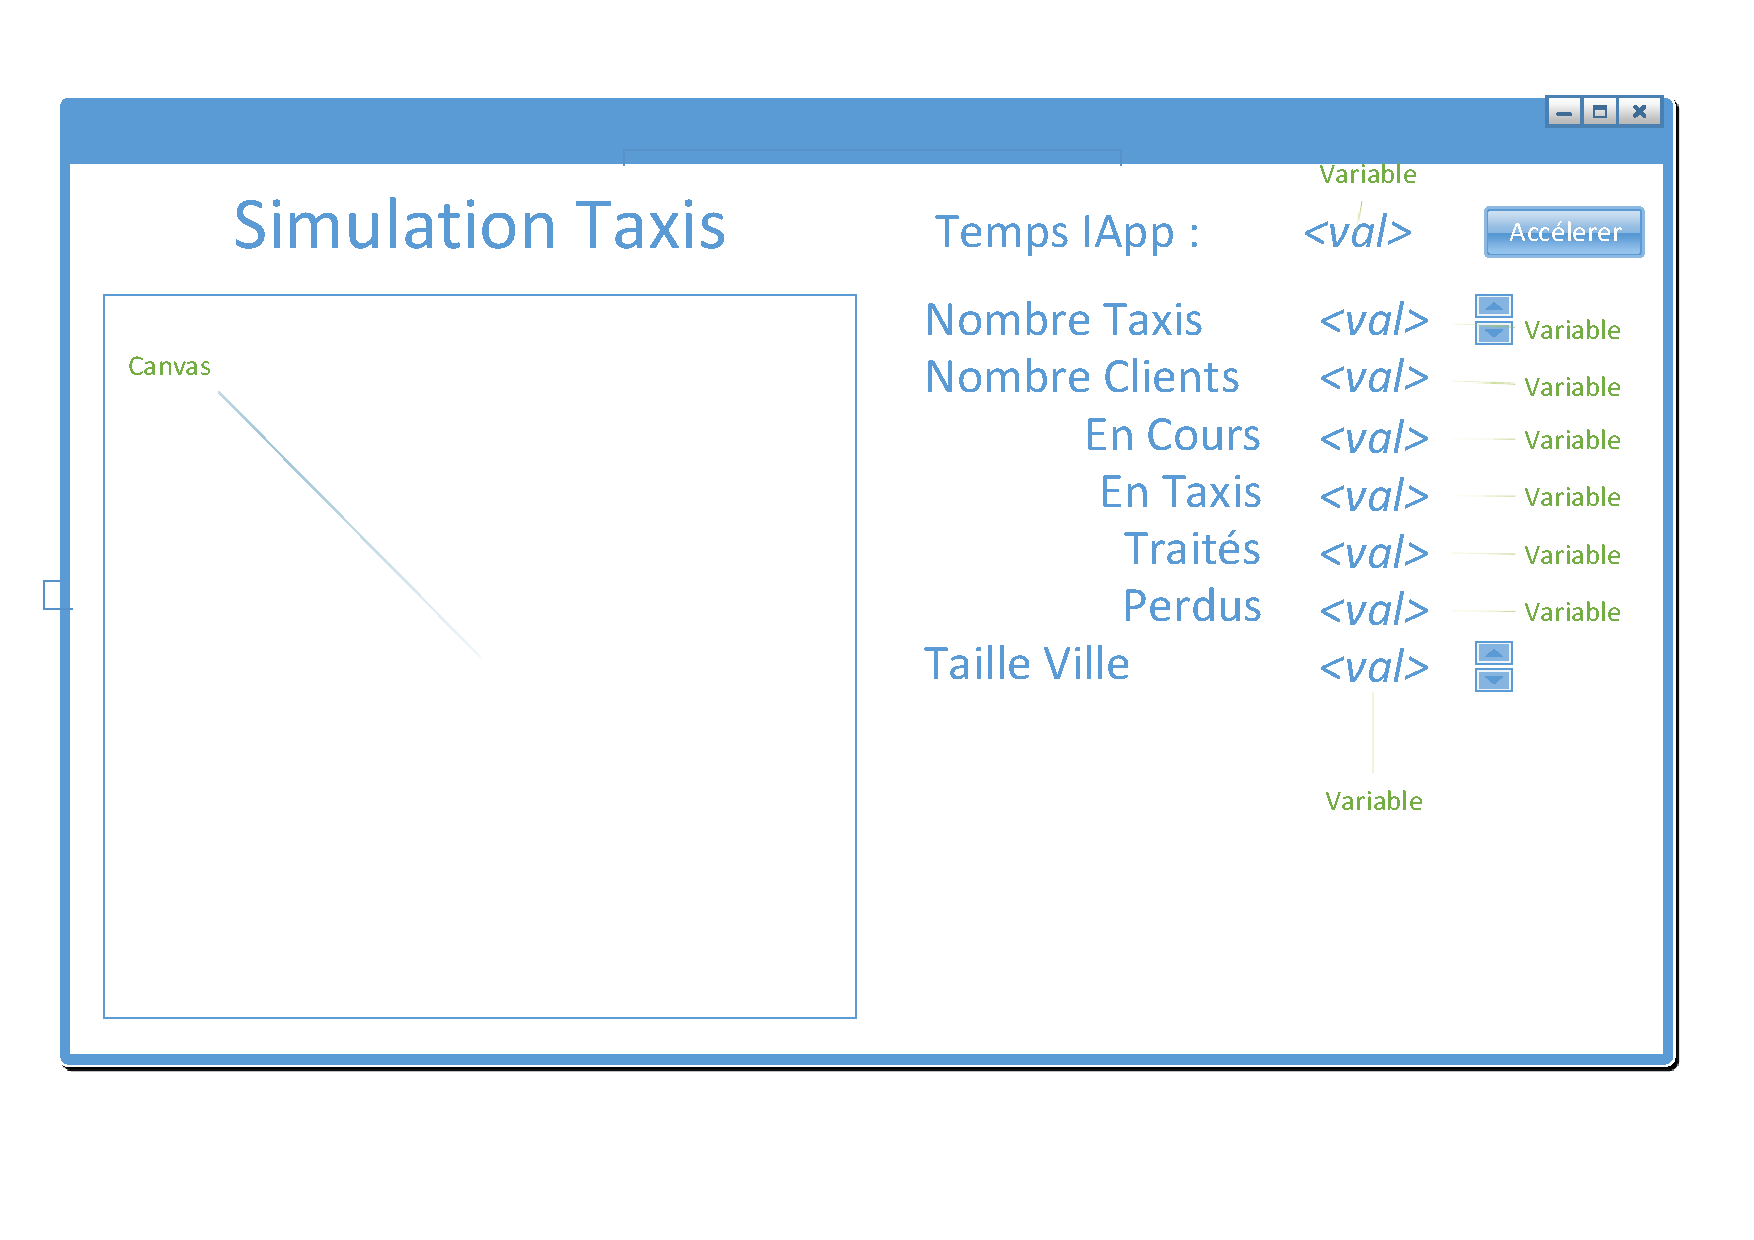
\includepdf[landscape=true,pages=-]{diagrame.pdf}


\end{document}
